\documentclass[
   12pt, % Schriftgröße
   DIV=calc,
   ngerman, % für Umlaute, Silbentrennung etc.
   a4paper, % Papierformat
   oneside, % einseitiges Dokument
   titlepage, % es wird eine Titelseite verwendet
   parskip=half, % Abstand zwischen Absätzen (halbe Zeile)
%   headings=normal, % Grˆfle der Überschriften verkleinern
   listof=totoc, % Verzeichnisse im Inhaltsverzeichnis aufführen
   bibliography=totoc, % Literaturverzeichnis im Inhaltsverzeichnis aufführen
   index=totoc, % Index im Inhaltsverzeichnis aufführen
%   captions=nooneline, % Beschriftung von Tabellen unterhalb ausgeben
   final, % Status des Dokuments (final/draft)
   numbers=noenddot
]{scrartcl}

%Abstände ändern
%\renewcommand*{\chapterheadstartvskip}{\vspace{-1\baselineskip}} %Abstand vor Section
\setlength{\headsep}{30pt} %Abstand Kopfzeile Textkörper

\usepackage{graphicx}

% !TEX root = ../Grunddatei.tex
%Wenn die Texte Umlaute oder ein Esszet enthalten, muss der folgende           Befehl bereits an dieser Stelle aktiviert werden:            %\usepackage[latin1]{inputenc}


\newcommand{\art}{AAI - Project documentation}
\newcommand{\titel}{Detection of one-way streets in satellite images}
\newcommand{\fachgebiet}{Applied Artificial Intelligence (I030)}
\newcommand{\autor}{Janico Nicke, Lukas Hauswald}
\newcommand{\supervisor}{Dr. Fouad Bahrpeyma}
\newcommand{\jahr}{2026}
\newcommand{\ort}{University of Applied Sciences Dresden}
\newcommand{\faculty}{Faculty of Informatics / Mathematics}
\newcommand{\logo}{Pictures/HTW_GESAMTLOGO_CMYK.pdf} %Informationen über das Dokument

\input{Metadaten/Packages.tex} %benötigte Packages
 
\makeindex

\input{Metadaten/page_style.tex} %Kopf- und Fußzeilen, Seitenränder..

%Hier beginnt das eigentliche Dokument
\begin{document}

\setcounter{secnumdepth}{3}
\setcounter{tocdepth}{3}

% !TEX root = ../Grunddatei.tex
\thispagestyle{plain}
\begin{titlepage}
	\begin{center}
		\vspace*{2.5cm}
		\includegraphics[width=0.5\linewidth]{\logo}\\[1.25cm]
		\Large{\textbf{\art}}\\[1.5ex]
		\LARGE{\textbf{\titel}}\\[3.5ex]
		

		\normalsize
		\begin{tabular}{p{5.4cm}p{7cm}}\\
			authors:  & \quad \autor\\[1.2ex]
			module: & \quad \fachgebiet\\[1.2ex]
			university: & \quad \ort\\[1.2ex]
		\end{tabular}
		
		\copyright\ \jahr\\[9ex]
	\end{center}
	
	%\singlespacing
	%\small
	%\noindent Dieses Werk einschliefllich seiner Teile ist \textbf{urheberrechtlich geschützt}. Jede Verwertung außerhalb der engen Grenzen des Urheberrechtgesetzes ist ohne Zustimmung des Autors unzulässig und strafbar. 
	%Das gilt insbesondere für Vervielfältigungen, Übersetzungen, Mikroverfilmungen sowie die  Einspeicherung und Verarbeitung in elektronischen Systemen.
	
\end{titlepage} %Deckblatt

%\include{Inhalt/Abstract} %Falls ein Abstract eingefügt werden soll

\pagenumbering{gobble}
 
\pagenumbering{Roman}

\tableofcontents %Inhaltsverzeichnis

% !TEX root = Grunddatei.tex
\addsec{List of Abbreviations}
\begin{acronym}[laaaaaaaaaaang] 
%In der Eckigen Klammer muss das längste Akronym stehen. 
%Es wird dann die gesamte weitere Tabelle danach ausgerichtet.
\end{acronym} %Abkürzungsverzeichnis

\newpage
\listoffigures % Abbildungsverzeichnis
\newpage
\listoftables % Tabellenverzeichnis
 
\clearpage

% 1.5-fachen Zeilenabstand
\onehalfspacing

% Text includes

\pagenumbering{arabic}
% !TEX root = Grunddatei.tex
%Hier können die einzelnen Kapitel hinzugefügt werden
%Sie müssen in den entsprechenden .TEX-Dateien vorliegen. 
%Die Dateinamen können natürlich angepasst werden.

% !TEX root = ../Abschlussarbeit_EN.tex
\section{Introduction}

For many people getting quickly and comfortably from A to B is a huge part of
their daily schedules.
Given the varied ways of transportation either by bike, bus, tram or car as
well as the underlying regulations and infrastructure a complex and multi-layered
traffic system is created.
To ensure effective and functional traffic management extensive data about a
given area is essential for numerous applications for example route finding,
real-time navigation or availability of different paths.
This is particularly relevant when looking at new technologies such as autonomous
driving.
Here, the vehicle needs great amounts of detailed data to successfully analyse
its environment so that safe and reliable travel can be guaranteed.
Remote sensing methods, especially the analysis of satellite imagery, are often
used in this context, to get valuable information about traffic infrastructure
and its surrounding area. Using the aerial view, many environmental features can
be detected, for example structures like roundabouts or intersections. Although
many attributes can be examined, this perspective also has its limits,
especially when looking at smaller traffic features, such as street signs or
road inclinations. To overcome this limitation, other technologies are used to
get information about the surrounding area from different perspectives.
Examples of that are radar-based concepts like LIDAR or images at ground level,
like street view images, which provide 360 degree images at a given location.

With remote sensing and complementary technologies providing increasingly
complex data for traffic management, the tools to analyse this information have
undergone substantial developments in recent years.
Since the launch of \textit{OpenAI’s ChatGPT} at the end of 2022, many
industries as well as research areas have seen rapid, ongoing developments when
using artificial intelligence (AI).
The technology can be found in almost every domain, for example in chatbots, AI
assistants or as a support tool in analysing different types of data.
The integration of different tools and models can be seen not only in IT, but
also in medicine, administration as well as transportation. For example, the
\textit{Fraunhofer IOSB-INA} is conducting research in traffic flow optimization using
AI technologies, as part of the \textit{AI4LSA} project \cite{FIOSBINA}.

In this project, we aim to combine environmental traffic data from different
sensing perspectives with artificial intelligence and deep learning methods,
to identify one-way streets at a given location. To determine the type of a
given street, the analysis is based on the detection of street signs, as they
are one of the primary indicators of one-way streets.
For that, the main approach is to analyse satellite images and street view
panoramas at intersections, using different AI models and techniques.


 
\newpage
% !TEX root = ../Grunddatei.tex
\section{Related works}

When looking at the domain of remote sensing, the inclusion of artificial intelligence is advancing rapidly. When searching for “satellite image” and “deep learning” on the research-sharing platform \textit{arXiv.org}, the number of published articles exceeds one hundred in 2025 alone. The developments in image analysis using artificial intelligence can improve existing use cases as well as introduce new ones. A small section of related articles will be presented in this chapter and can be seen as representative for other related works.

At the 17th Python in Science Conference in 2018, Virginia Ng and Daniel Hofmann presented a methodology to implement scalable tools for extracting features in remote sensing images, using deep learning methods. The proposed approach can be used for a variety of tasks, for example object detection, segmentation and feature mapping. It also covers various features, ranging from roads and bikes to bodies of water or even glacies. The paper includes an overview of the basic pipeline, that includes the data preparation as well as implementation of different deep learning models such as U-Net or YOLO. The authors also presented specific adaptations of the methodology for the aerial and satellite imagery domain. Last, they discussed further efforts to improve the proposed deep learning models, so that new applications can also be covered \cite{relWork1}.

The second paper, written by Lei He et al, propose an improved deep learning approach for accurate road segmentation from remote sensing imagery. Due to the improved segmentation precision and reduced computational complexity, the new technology can be used to extract roads from satellite imagery. The authors introduce a modified architecture called D-DenseNet, which includes parts of both D-LinkNet and DenseNet. The proposed approach demonstrates its suitability for precise and computationally efficient road extraction \cite{relWork2}.

Chenao Zhao et al challenge current models when faced with vehicle detection tasks in satellite imagery, by introducing a novel vehicle detection called SatDetX-YOLO. The new approach is based on YOLOv8 and is characterized by several architectural changes that stem from combinations with other models. For instance, the model includes a backbone network with FasterNet as well as a Deformable Attention Module. When comparing the results between different models, a slight increase in accuracy, precision, recall and mean average precision can be observed (around 3 percent respectively) \cite{relWork3}.

The last presented paper, by Andrew Campbell, Alan Both and Qian Sun, explores the possibilities of automated classification tasks in Google Street View images using machine learning technologies. Focus of their work lies on the detection of traffic signs. The authors developed a custom object detection model to classify certain street signs from images captured at intersections and get their approximate locations. The implementation shows notable detection and classification accuracies of around 96 and 98 percent respectively as well as the ability to be easily scalable. Due to those characteristics and the workflow using open-source data, the proposed solution shows great potential for real-world applications \cite{relWork4}.

From what we can infer, our approach is relatively novel, as we could not find articles that follow a similar approach for one-way street identification. Although, a lot of research has been done for satellite images and street view panoramas respectively, combined solutions using both seem rather unique. The same appears to be true for segmentations of road intersections in satellite imagery, which seems to be a less explored research topic. 
\newpage
% !TEX root = ../Grunddatei.tex
\section{Methodology}

\subsection{Goals and tasks}
In this project, our main goal is to examine the potential and the limits of street analysis for freely available data sources. Those include open-source remote sensing data, specifically satellite images, as well as free ground-level imagery of streets and their surroundings. We aim to apply computer vision methods and technologies to detect street features, so that information about an area can be obtained and used for further analysis. The core of this project is to design and implement a workflow to connect satellite images, ground-level street view panoramas and deep learning systems in a combined automated application. For this, the project explores nuances of model capabilities in a combined setting, especially when given data (like satellite images or street view images) of varying quality.

As described, the main objective of this project is to create an application to automatically detect one-way streets in satellite imagery, based on ground-level views of found intersections. For that, we want to use different deep learning methods to approach the individual tasks. These include three major steps that can be used to group the different subtasks. The first task is the detection of an intersection in a given satellite image. The main purpose for this is to segment the area occupied by the intersection. This can be used in the second task, which includes the extraction of a street view panorama at the found intersection. Third, this 360-degree image is analysed for relevant sections of the panorama. Last, the detection of street signs relevant for one-way streets concludes the application.

\subsection{Used technologies}
A number of different tools, models and data sources are used to implement the individual tasks of the application. To get satellite images, the open-source remote sensing platform MapTiler is utilised. This service provides online maps, including satellite imagery of varying resolution, maps for data visualisation or schematic maps for specific use cases. For the proposed workflow, the \textit{MapTiler API} is used to get map tiles that can be combined into satellite images with a resolution of around 20cm per pixel \cite{Maptiler1}. The company offers a free access plan for non-commercial use that includes 100.000 API calls per month \cite{Maptiler2}. To get open-source street view panoramas, we are using \textit{Panoramax}, an open-source project dedicated to collecting and providing street level imagery. The free alternative to Google Street View was first founded by the French National Geographic Institute and includes over 74 million images, mostly focusing on French national territory. The project includes different instances that mostly provide different data. Each of those instances have individual API endpoints that are primarily used to search for, filter or download images and other data \cite{3panoramax}. In this project, the service is utilised to automatically locate and download 360-degree images at intersections that are detected in satellite images. Due to the data being geographically confined, the proposed workflow is developed and tested in a limited area. For this, we chose the French city of Caen, because of the density of available data in this region. Figure~\ref{fig:panoramax} shows the density of 360-degree panoramas available at Panoramax in Caen, Figure~\ref{fig:svp} illustrates an example for a specific street view panorama.

\begin{figure}[htbp]
    \centering
    
    \begin{minipage}{0.48\textwidth}
        \centering
        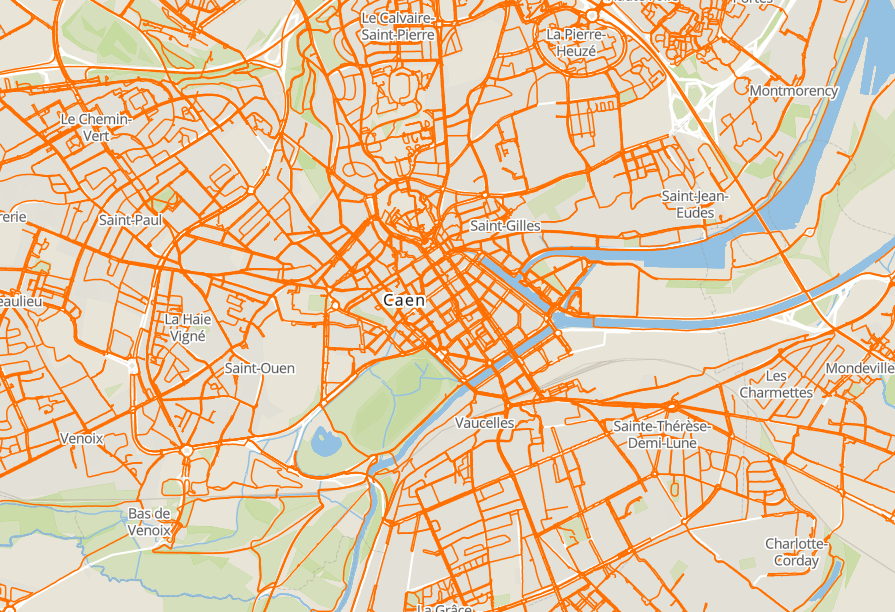
\includegraphics[width=\linewidth]{Pictures/panoramax_caen.png}
        \caption{Density of Panoramax street view images in Caen, France – source: api.panoramax.xyz}
        \label{fig:panoramax}
    \end{minipage}
    \hfill
    \begin{minipage}{0.48\textwidth}
        \centering
        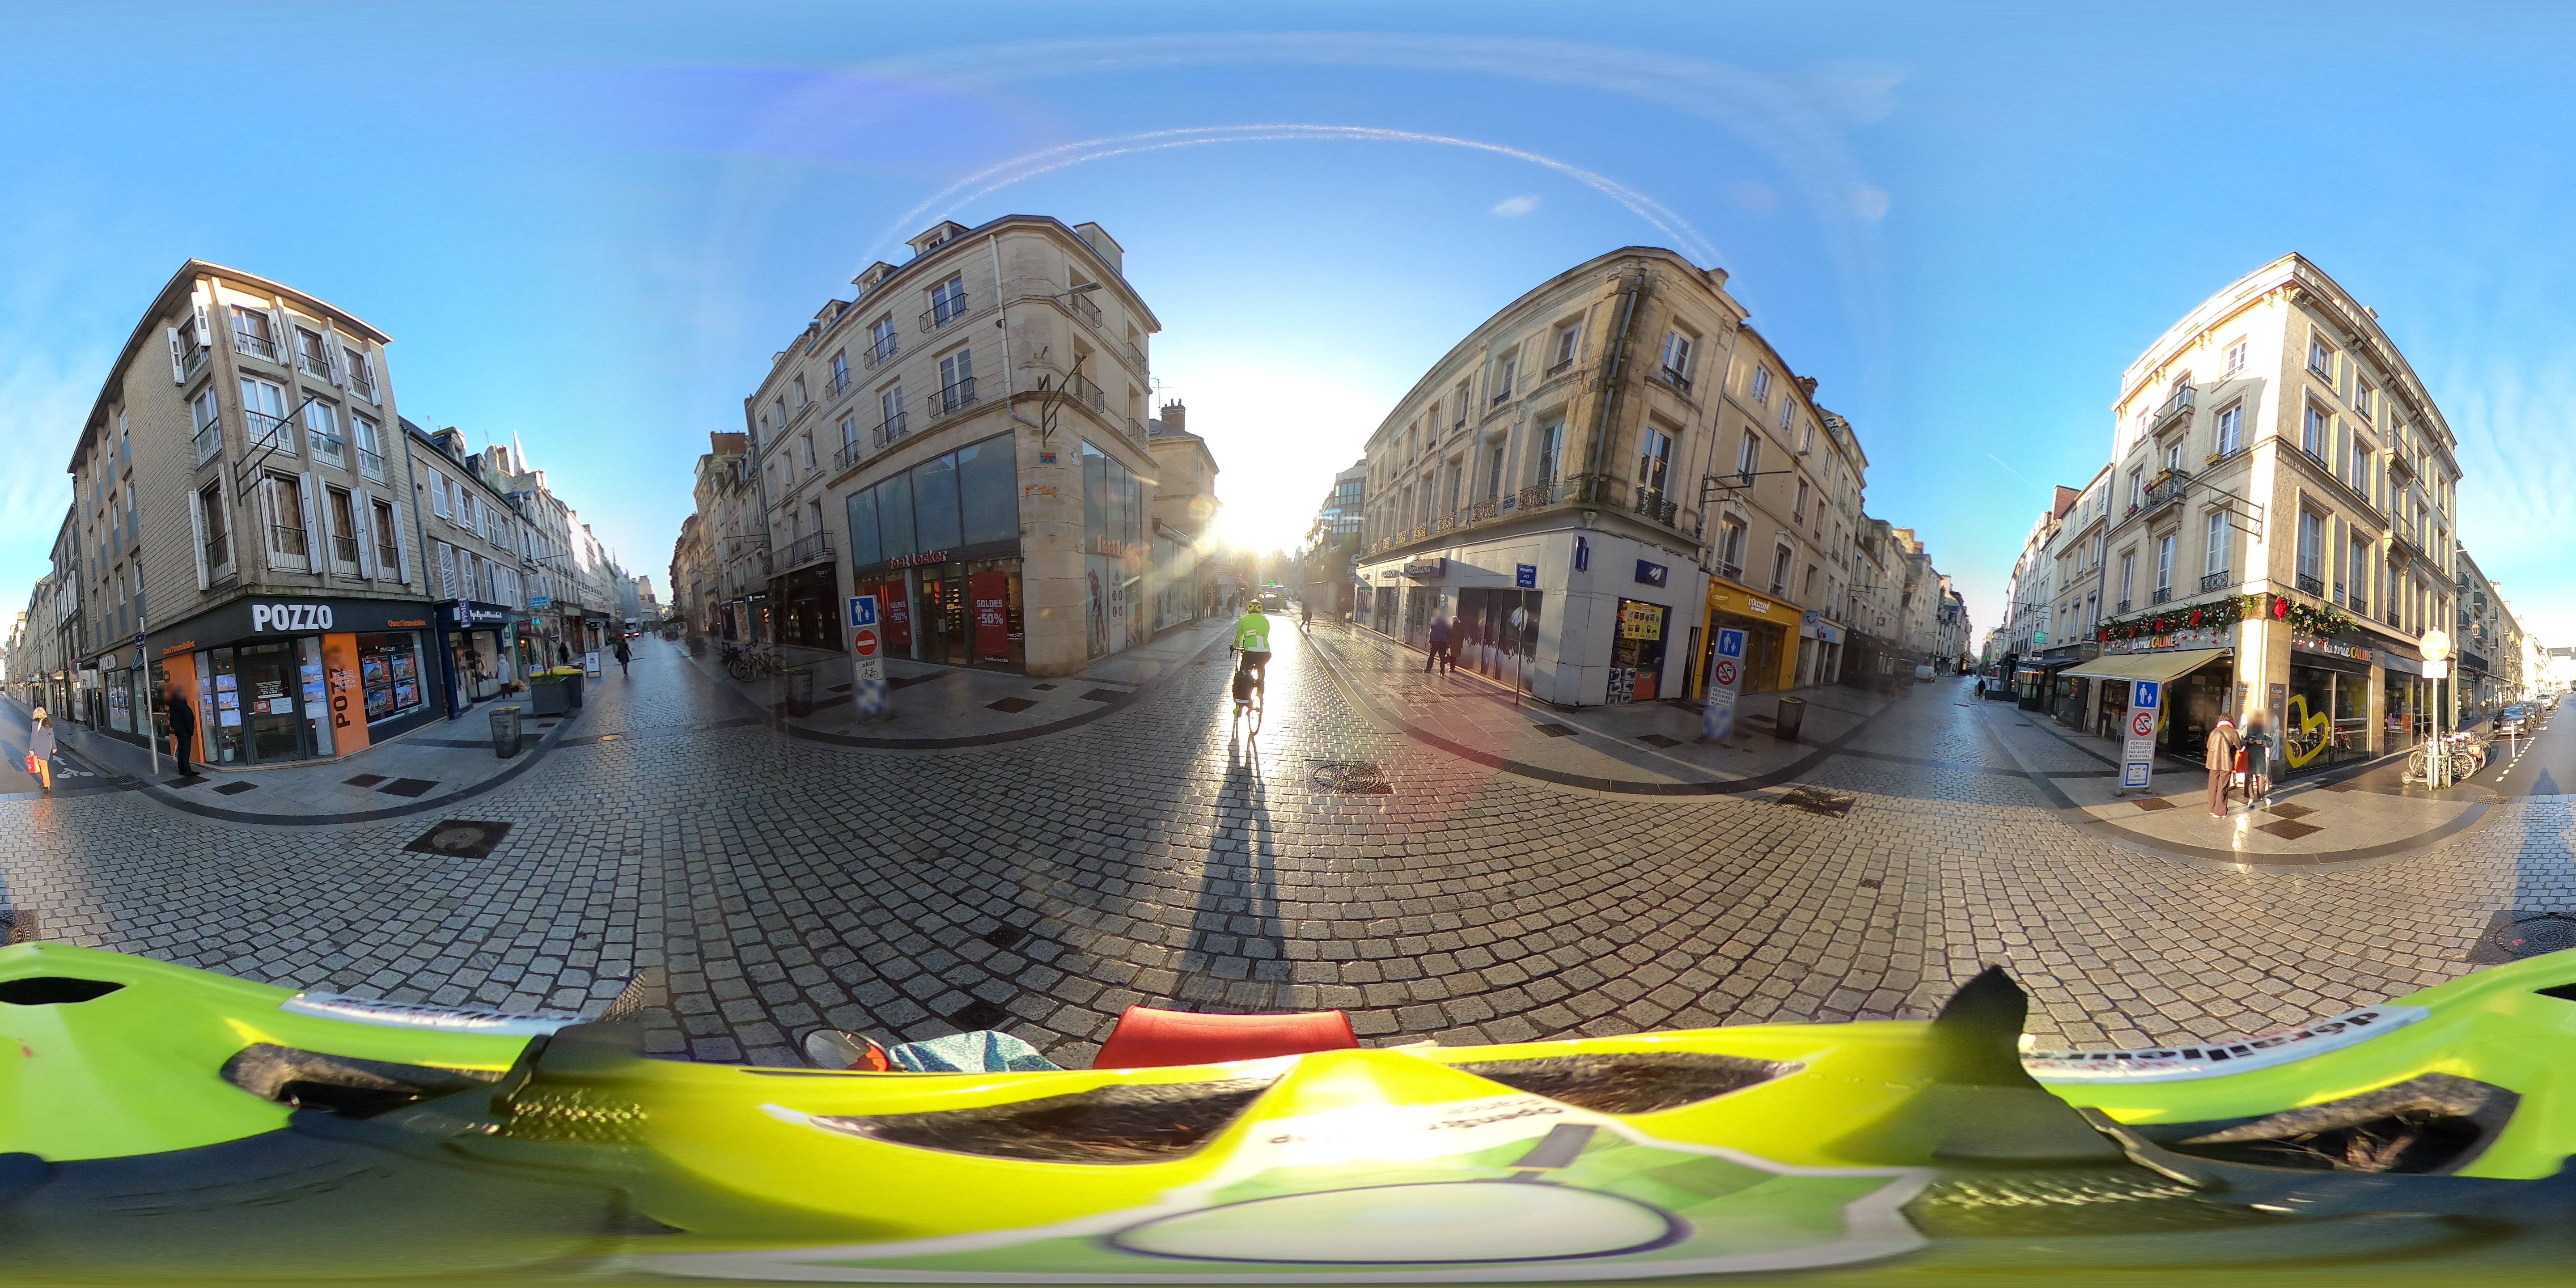
\includegraphics[width=\linewidth]{Pictures/svp_example.jpg}
        \caption{Example for street view panorama – source: api.panoramax.xyz, user: AlbaireN (uploaded 16.01.2025)}
        \label{fig:svp}
    \end{minipage}
    
\end{figure}

To analyse the collected images, the \textit{YOLO11} model by Ultralytics is used for the segmentation and detection task of the application. The model is characterised as an extension of classic convolutional neural networks that are often used for classic computer vision tasks, like object detection, classification or segmentation. The advancements of this technology are primarily because of changes in model architecture and lead to a very high computation and prediction speed while maintaining good accuracy \cite{4ultralytics}. Another factor for choosing YOLO11 for this project is the easy integration of the model into automated workflows as well as the results that get produced when running inference. Here, the produced data of segmentation and classification tasks include coordinates to identify relevant areas of a given image, which can be easily utilised for subsequent tasks. Another model called \textit{Depth Anything V2} is used for identifying relevant sections of the panorama image from Panoramax. This application is used to obtain a monocular depth estimation by producing a depth map of a given image \cite{5depthAnything}.

Other technologies are used in this project for creating custom datasets. The open-source platform \textit{Label Studio} is used to annotate data for machine learning processes \cite{6labelstudio}. To correctly segment intersections in the provided satellite images, we created a dataset containing 99 images with labelled intersection areas, which is used to fine-tune the applied YOLO11 model. To obtain the needed satellite images of intersections, we used a dataset from the French government office DINUM that included a detailed list of all intersections in France and their location, ordered by the respective départements (French administrative districts) \cite{7DINUM}. To combine all the tasks as a coherent implementation of the workflow, we use the programming language python.

\subsection{Proposed workflow}

The following flowchart (Figure~\ref{fig:flowchart}) presents all (sub-)tasks of the proposed application.

\begin{figure}[htbp]
    \centering
    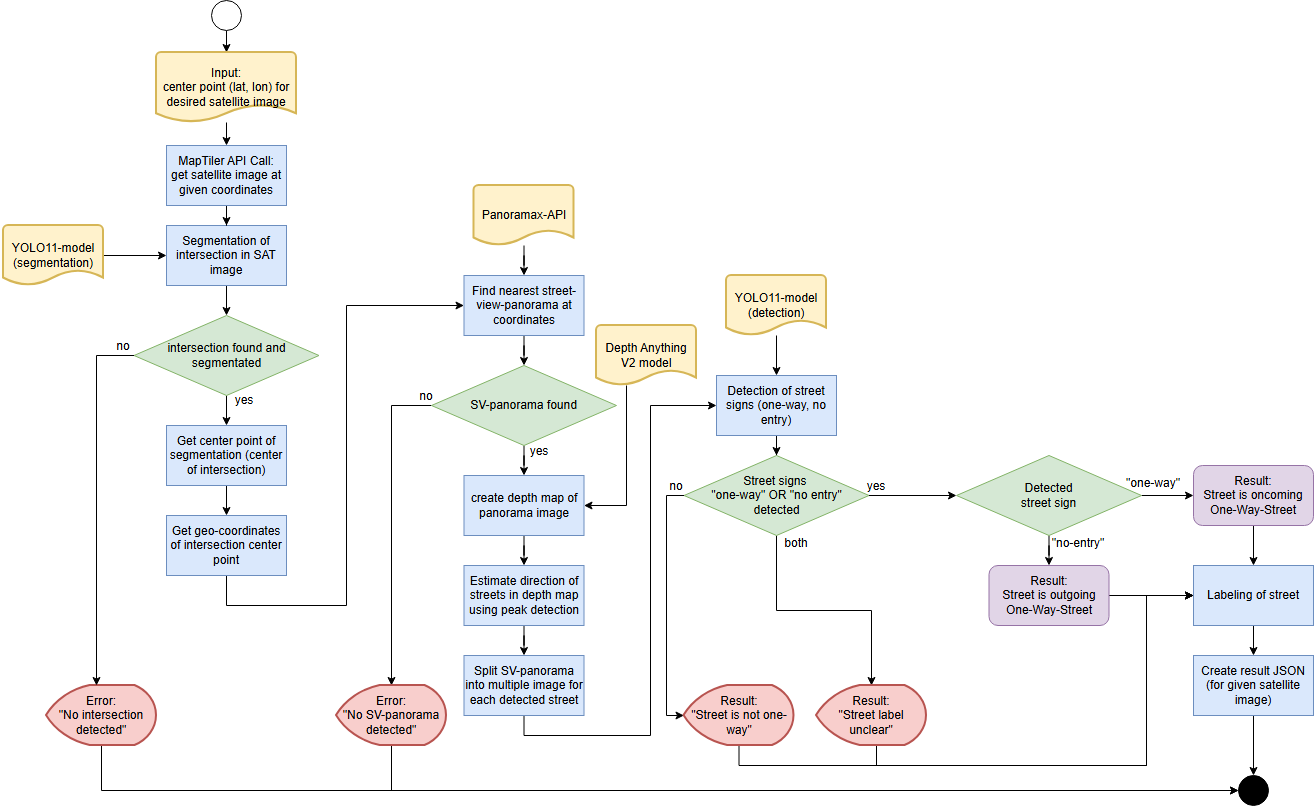
\includegraphics[width=\linewidth]{Pictures/flowchart.png}
    \caption{Flowchart of the proposed Workflow / Application – source: own depiction using draw.io}
    \label{fig:flowchart}
\end{figure}

The following section is dedicated to explaining specific subtasks of the application in further detail, starting with the identification of the intersection center point. For this, the output of the segmentation model (YOLO11) can be utilised. This YOLO11 model produces a polygon that represents the intersection area found in a given (satellite) image. This result is saved as a text file, which includes all coordinates of the segmentation polygon in the original image. Those coordinates represent specific normalised image pixels that define the edges of the polygon. Using this data, it is possible to obtain the mean value of the polygon, which represents the center point of the segmented area in the satellite image and thus, the center of the intersection. A comparison with the center point of the whole image allows the geographical coordinates of the intersection center point to be derived, since the image center always represents the provided coordinates from which the satellite image was formed. By calculating the distance, a single pixel corresponds to a real-world measurement and by determining the difference between both positions, it is possible to work out the coordinates of the segmentation center. A graphical depiction of the intersection center point detection is presented in Figure~\ref{fig:satImg_results}.

\begin{figure}[htbp]
    \centering
    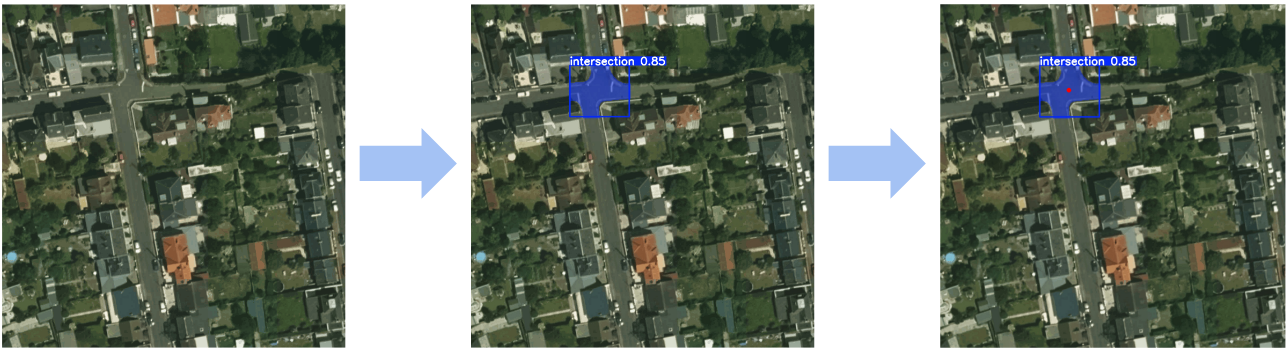
\includegraphics[width=\linewidth]{Pictures/satImg_results.png}
    \caption{Flowchart of the proposed Workflow / Application – source: own depiction using draw.io}
    \label{fig:satImg_results}
\end{figure}

SCHRITT FÜR DIE PEAK DETECTION

The other tasks can be implemented using simpler routines. For example, basic API requests with the python package \textit{requests} can be used to get data from individual MapTiler or Panoramax endpoints. This includes receiving satellite images and street view panoramas, as well as obtaining the nearest panorama image, given a specific location. The models included in the proposed workflow mostly require executing their respective prediction functions/commands with corresponding parameters. Last, saving the results of the analysis in JSON-files can also be done easily by utilising the python package \textit{json}.

\newpage
% !TEX root = ../Grunddatei.tex
\section{Experimental results}

To execute our tool you just need to go into the
\texttt{OneWayStreet\_analysis\_complete}-folder and execute \texttt{run.py}.
Before that you should give the tool writing access to this folder so it can
create the results and save them. You also probably need to create your own
API Key at  for the access to \textit{MapTiler} and insert it as \texttt{api\_key}.
You can set the coordinates as \texttt{lat\_sat, lon\_sat} at the top of the script
as well as choose your own identifier for the results. Another parameter
important for testing is the radius. This variable tells our program how far to
search for streetview panoramas.
We recommend to choose your test coordinates with care in
\texttt{https://panoramax.openstreetmap.fr/} and set as a filter 360° images only.
It is generally best to actually pick coordinates where there is only one
intersection visible and where there are actually usable streetview images.

After starting the program it will first download the image with the exact
coordinates given as center and with given zoom and tile radius from
\textit{MapTiler}.
Then it uses the \textit{YOLO11} model to get the center point of the
intersection in the image and return its coordinates as latitude and longitude.

These values can then be used to download the nearest streetview panorama from
the given panoramax instance. Currently there is no API Key needed to
download images from the instance in the code, so we recommend just using it.
If this instance should however not be responsive there are some other instances,
whose urls can be used instead.

After this our chosen street detection function is used to crop the streetview
panorama for separate streets.

Then again for every crop the \texttt{classify\_street}-function is used to
classify the street as explained in methodology.

As in between results the satallite image, the segmented satellite image,
the streetview panorama and the crops of the streetview panorama are written
to the file system.

As a final result the \texttt{summary.json} is saved, which contains some metainformation
about the panoramax image, the coordinates from the start, the intersection center point
and finally the angles of the roads detected inside streetview panorama with
their respective label. This result is machine readable and could be resused by
other functions.

The following section is about the results of each subtask and how well they
perform as parts of the proposed workflow.
The first step is getting a satellite image at given coordinates.
This step works flawlessly and can be done easily, since it only requires to
define latitude and longitude. During our work in this project, we also had no
problems with the \textit{MapTiler} API, as we could stay below the free limit.
It must be mentioned, that the quality of satellite images, while very good for
the area around Caen, can vary depending on the given coordinates.
This is, for example, because available data originates from different
satellites, that could have worse quality.

The results of the second step, the intersection segmentation, are also quite good.
When looking at the model training, both precision and recall are equal to around 0.8.
This means, that the current model is good at finding an intersection in a given
satellite image as well as segmenting its area.
Another metric for model quality is the mean average precision, which equals to
around 0.5.
This means, that the model is slightly worse at creating a very detailed
segmentation of the intersection. In practice this means, that the resulting
segmentation might not reflect the actual area of the intersection accurately
and instead, creates segmentation areas that are fuzzy or include small parts of
adjacent areas. Fortunately, the effects on our proposed workflow are minimal,
since we don’t need or use a very detailed segmentation of a given intersection
and only use it to estimate the center point.

Third, this estimation of the intersection center point as well as the following
download of an adjacent street view panorama from \textit{Panoramax} also works
faultless.
However, it must be mentioned that the download can still fail, depending on the
chosen search radius and the density of street view panoramas.
When looking at different areas, it could be needed to change this search radius
parameter.
During our test for Caen, the current value did not disrupt the current implementation.
The next step of our workflow is the identification of relevant sections of a
given street view panorama.
The results show, that the proposed approach works in principle, but still needs
fine tuning.
During our tests, we only achieved a precision of 65.79 \% and a recall of
around 53 \%.
The F1-Score of our solution equals to 57.45 \%.
A reason for the current flaws is that the used street view panoramas can vary
immensely. Different shortcomings are, for example, a disparate recording angles
as well as the complexity of a given intersection scene, that can include
different buildings, structures, participants or other objects.
The current implementation does not account for all of those influences, which
is why irrelevant sections of the panorama might be identified incorrectly,
which impacts the continued workflow and the end results.

The fourth step is the detection of street signs in images that represent the
relevant sections of the streetview panorama. Our tests show, that the current
implementation produces accurate results and can be used as intended in our
proposed workflow. Here, the developers of the used models published own metrics
of their respective models on \textit{Hugging-Face}.
The \texttt{Panoramax/detect\_face\_plate\_sign}-model has a provided accuracy for
road signs of 0.879 which is still very high and the
\texttt{Panoramax/classify\_fr\_road\_signs}-model for classification has an
accuracy of 0.987. These results match our own tests during this project.

The last step of creating a results JSON file as well as all additional
(auxiliary) functions work flawlessly and produce the necessary data needed for
the following subtasks of the proposed workflow.



\newpage
% !TEX root = ../Grunddatei.tex
\section{Conclusion}

The results shown indicate that the proposed workflow can be used to detect
one-way streets, by combining satellite imagery, street view images and modern
deep learning technologies. The presented application is able to produce
meaningful and accurate results that can be used for further analysis.

However, the current workflow also introduces some limitations and challenges. First, the approach and implementation lean heavily on the existence of available, high-quality image data at a given location. Since streets and their surrounding environment are highly complex frameworks, it can be possible that the image quality is insufficient for an effective segmentation of intersections and thus, the entire analysis. It is also possible for the available satellite images to stem from system that can only offer low-resolution imagery, which would limit the quality and accuracy of the procedure. Another limiting factor is that, as discussed, Panoramax are mostly restricted to French territory. Since the application uses 360-degree images, it is obvious that the proposed workflow does not work in areas with low density of street view panoramas. To address this issue, other services, like Google Street View, could be included, although that would most likely mean including proprietary data sources.

Further development of the approach could include refining the current implementation or model architecture to achieve more accurate results that are less vulnerable to errors. It is also possible to test and expand the workflow for other areas, cities or countries. Another advancement could be to more accurately represent different edge cases and make the application more resilient to the complex nature of road environment analysis.

% Literaturverzeichnis 
\bibliography{Bibliographie} % Aufruf: bibtex Bibliographie.bib
\bibliographystyle{natdin} % DIN-Stil des Literaturverzeichnisses


% Ende des Dokuments
\end{document}
%------------------------------------------